\section*{IV. Kết quả Thực nghiệm \& Đối chuẩn}

\subsection*{Bảng Chỉ số Hiệu năng Đối chuẩn Toàn diện}
Bảng dưới đây tổng hợp và đối chuẩn chi tiết các chỉ số hiệu năng cốt lõi giữa hai cấp độ mô hình: \textbf{Snapshot Tĩnh} (khảo sát tại tọa độ danh định $q_U^{(0)} = (0.5, 0.4)$) và \textbf{Hành trình Động học} ($N=10$ khe thời gian). Các mốc cơ sở (Baseline) được phân định rõ ràng nhằm phản ánh chính xác tỷ lệ cải thiện hiệu năng:

\vspace{0.2cm}
\begin{center}
\renewcommand{\arraystretch}{1.25}
\begin{tabularx}{\textwidth}{|X|>{\centering\arraybackslash}m{2.3cm}|>{\centering\arraybackslash}m{2.3cm}|>{\centering\arraybackslash}m{2.3cm}|>{\centering\arraybackslash}m{2.5cm}|}
\hline
\rowcolor{tableheader}
\textbf{Chỉ số Đánh giá (Metric)} & \textbf{Snapshot Tĩnh: AO Tĩnh} & \textbf{Hành trình Động: Trước Tối ưu} & \textbf{Hành trình Động: AO Động ($N=10$)} & \textbf{Hành trình Động: DRL DDPG} \\
\hline
Cấu hình không gian & Tọa độ tĩnh $q_U^{(0)}=(0.5, 0.4)$ & Quỹ đạo thẳng $q_{\text{start}} \to q_{\text{end}}$ & Tối ưu luân phiên SQP/Penalty & Học tăng cường Actor-Critic \\
Phân bổ công suất $\alpha_1$ & $\alpha_1^{(0)} = 0.75 \to 0.795$ & Cố định $\alpha_1 = 0.75$ & Động $\alpha_1^*[n] \in [0.77, 0.83]$ & Động $\alpha_1^*[n] \in [0.78, 0.83]$ \\
\hline
Xác suất dừng TB ($\bar{P}_{\text{out}}$) & $0.0701 \to \mathbf{0.00533}$ & $0.0401$ (BM3: $0.0481$) & $\mathbf{0.0206}$ & $\mathbf{0.0197}$ \\
Xác suất dừng xa $D_1$ & $0.0463 \to 0.00318$ & $0.0245$ & $0.0098$ & $0.0089$ \\
Xác suất dừng gần $D_2$ & $0.0249 \to 0.00216$ & $0.0160$ & $0.0109$ & $0.0110$ \\
\hline
Mức giảm xác suất dừng & \textbf{Giảm 92.4\%} (vs $0.0701$) & Baseline ($0\%$) & \textbf{Giảm 48.6\%} (BM3: $57.2\%$) & \textbf{Giảm 50.9\%} (BM3: $59.0\%$) \\
Thời gian tính toán / suy luận & $120.0$ ms & N/A & $1\,850.0$ ms (tổng 10 khe) & $\mathbf{1.5}$ \textbf{ms/khe} ($15$ ms tổng) \\
Số vòng lặp / tập hội tụ & $5$ vòng lặp & N/A & $4$ vòng lặp & $\approx 50$ episodes \\
Tỉ lệ vi phạm an toàn SIC & $\mathbf{0.0\%}$ (đệm an toàn) & $0.0\%$ (cố định) & $\mathbf{0.0\%}$ (đệm $0.10$) & $\mathbf{0.0\%}$ (đệm $0.06$) \\
Khả năng điều khiển trực tuyến & Ngoại tuyến & Không & Ngoại tuyến & \textbf{Trực tuyến (Real-time)} \\
\hline
\end{tabularx}
\end{center}
\vspace{0.2cm}

\subsection*{Quan sát Định lượng Cốt lõi}
\begin{itemize}[leftmargin=1.5em]
    \item \textbf{Phân định rõ ràng giữa hai mốc tham chiếu cơ sở (Baseline):} 
    (1) Đối với mô hình Snapshot Tĩnh tại tọa độ danh định $q_U^{(0)}=(0.5, 0.4)$ với $\alpha_1=0.75$, xác suất dừng trước tối ưu là $0.0701$, sau tối ưu giảm xuống $0.00533$ (mức suy giảm đạt $92.4\%$).
    (2) Đối với mô hình Hành trình Động qua $N=10$ khe thời gian, mốc trước tối ưu tương ứng với đường bay thẳng từ $q_{\text{start}}$ đến $q_{\text{end}}$ với công suất cố định $\alpha_1=0.75$ có xác suất dừng trung bình là $0.0401$ (hoặc $0.0481$ đối với kịch bản Benchmark 3 không tối ưu cả vị trí và công suất). Cả thuật toán AO Động và tác tử DRL đều giảm xác suất dừng về vùng xấp xỉ $\approx 0.02$ (AO đạt $0.0206$ - giảm $48.6\%$, DRL đạt $0.0197$ - giảm $50.9\%$).
    \item \textbf{Tính nhất quán toán học theo công thức dừng hệ thống:} Toàn bộ số liệu trong Bảng đều thỏa mãn nghiêm ngặt điều kiện xác suất dừng toàn phần $OP_{\text{total}} \ge \max(OP_{D1}, OP_{D2})$ theo đúng công thức xác suất hợp \eqref{eq:op_total_exact}.
    \item \textbf{Xác thực công thức giải tích Marcum-Q:} Kết quả mô phỏng Monte-Carlo với $10^5$ mẫu (ký hiệu hình tròn đen `ko' trên Hình \ref{fig:ao_static_snr}) phù hợp chặt chẽ với đường cong giải tích Marcum-Q trong phạm vi sai số thống kê cho phép trên toàn dải SNR từ $10 \to 26$ dB (tại $OP \approx 10^{-3}$, sai số thống kê lý thuyết của $10^5$ mẫu là khoảng $10\%$).
    \item \textbf{So sánh khách quan giữa DRL và AO theo quy ước khe thời gian:} 
    (1) \textit{Ảnh hưởng của quy ước khe:} Trong AO, quỹ đạo được tối ưu qua 10 nút mốc rời rạc với $q_1 = q_{\text{start}}$ và $q_{10} = q_{\text{end}}$ (tương ứng 9 bước di chuyển). Khe $n=1$ của AO được tính tại đúng điểm xuất phát $q_{\text{start}}(0.35, 0.50)$ cách xa người dùng nên $OP[1] \approx 0.1008$. Trong khi đó, tác tử DRL xuất phát tại $q_{\text{start}}$ ở $t=0$ và thực hiện 10 bước chuyển động, trong đó $OP[n]$ được tính sau mỗi bước (ở bước $n=1$, UAV đã dịch chuyển đến $(0.47, 0.435)$ gần người dùng hơn, dẫn đến $OP[1] \approx 0.0672$). Độ chênh lệch $\approx 0.0336$ tại khe 1 chia bình quân 10 khe đã đóng góp mức chênh lệch $\approx 0.0034$ vào xác suất dừng trung bình.
    (2) \textit{Hiệu năng tại các khe ổn định:} Tại các khe giữa ($n=5 \to 8$), giải thuật SQP của AO duy trì vị trí tối ưu ổn định ở $(1.105, 0.200)$ và đạt xác suất dừng $OP \approx 0.0053$, nhỉnh hơn so với mức $0.0056 - 0.0060$ của tác tử DRL. Điều này khẳng định AO đóng vai trò là cận tham chiếu chuẩn số học (numerical benchmark), trong khi DRL đạt hiệu năng bám sát cận chuẩn này.
    (3) \textit{Ưu thế quyết định của DRL:} Ưu thế then chốt của DRL nằm ở tốc độ suy luận trực tuyến $\mathbf{1.5}$ ms/khe (nhanh hơn $120$ lần so với thời gian giải lặp $1\,850$ ms của AO), cho phép triển khai điều khiển thời gian thực trên bo mạch UAV.
\end{itemize}

% -------------------------------------------------------------------------
\subsection*{1. Kết quả Mô phỏng Tối ưu hóa Luân phiên Tĩnh}
Mô hình AO Tĩnh thực hiện khảo sát tại một khe thời gian danh định (snapshot) nhằm kiểm chứng cơ sở toán học và đặc tính hội tụ cơ bản:

\begin{figure}[H]
    \centering
    \begin{subfigure}[b]{0.49\textwidth}
        \centering
        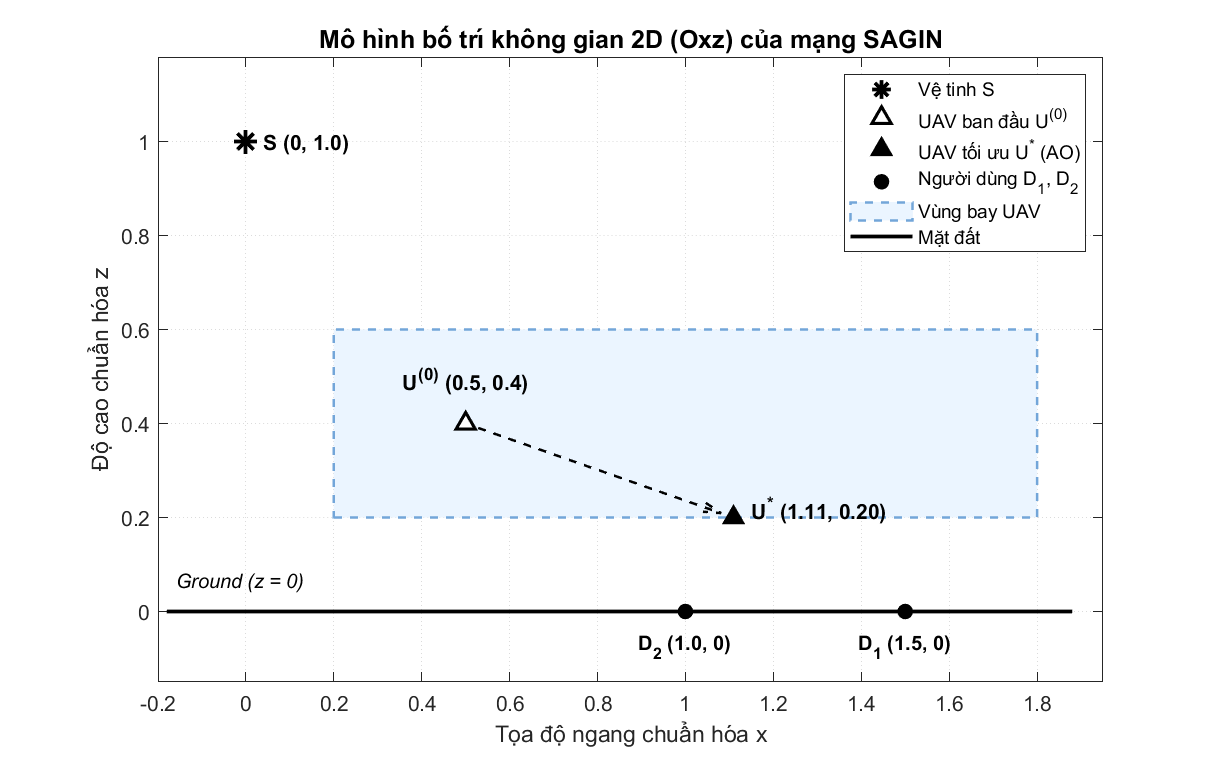
\includegraphics[width=\textwidth]{figures/ao_static_fig3_trajectory.png}
        \caption{Vị trí tĩnh tối ưu của UAV trong mặt phẳng 2D $(Oxz)$}
        \label{fig:ao_static_pos}
    \end{subfigure}
    \hfill
    \begin{subfigure}[b]{0.49\textwidth}
        \centering
        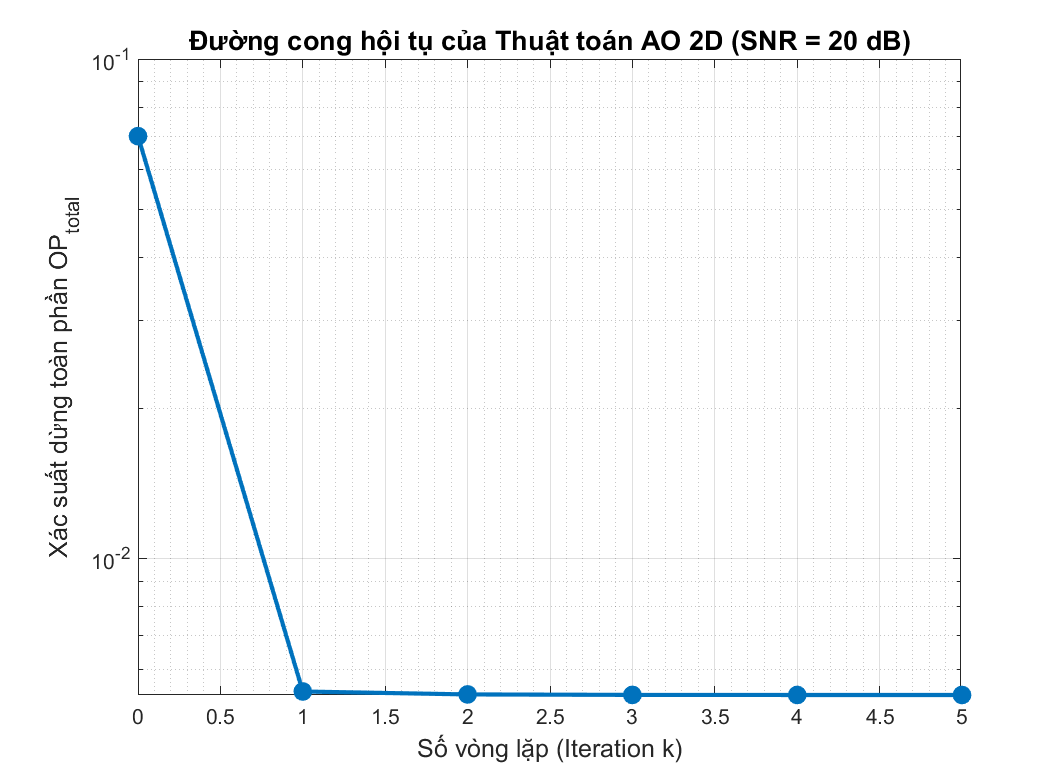
\includegraphics[width=\textwidth]{figures/ao_static_fig1_convergence.png}
        \caption{Đặc tính hội tụ của thuật toán AO tĩnh qua 5 vòng lặp}
        \label{fig:ao_static_conv}
    \end{subfigure}
    \caption{Kết quả vị trí không gian tĩnh và đặc tính hội tụ đơn điệu của giải thuật AO tĩnh.}
    \label{fig:ao_static_group1}
\end{figure}

\begin{figure}[H]
    \centering
    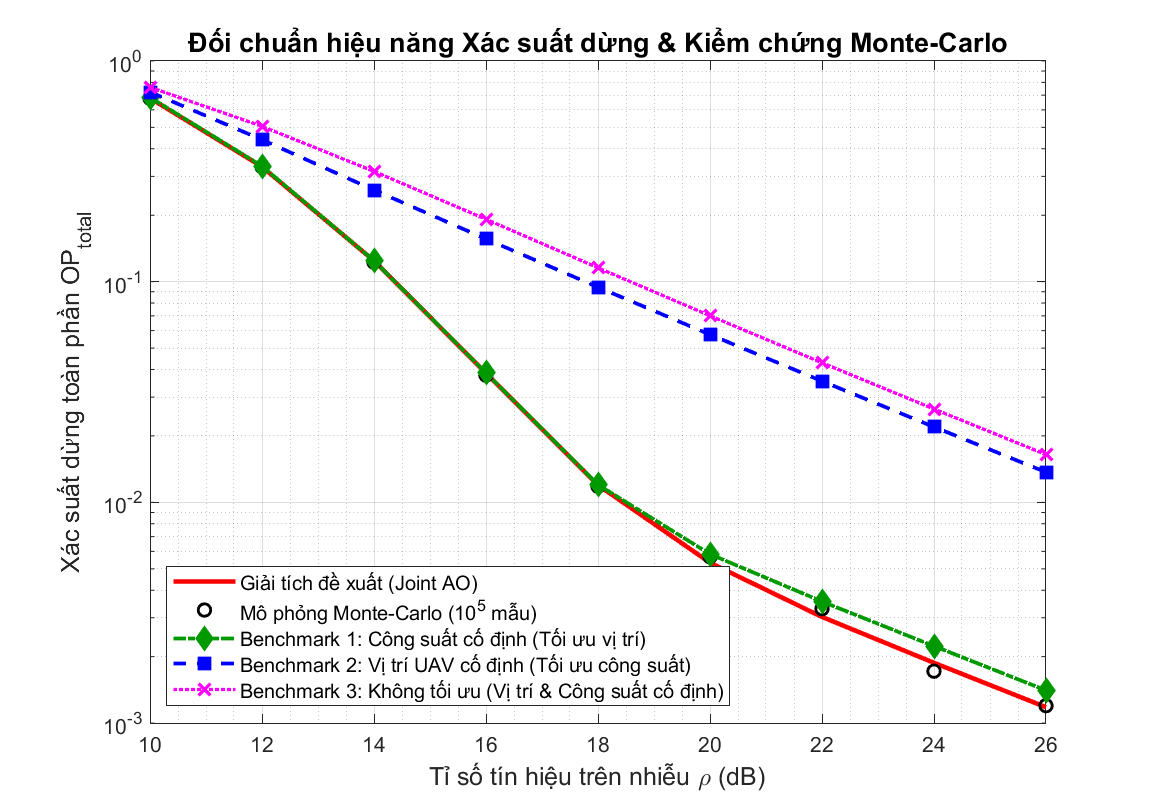
\includegraphics[width=0.72\textwidth]{figures/ao_static_fig2_snr.png}
    \caption{Đối chuẩn xác suất dừng qua dải SNR chuẩn hóa $\rho = \bar{\gamma}_S = \bar{\gamma}_U$ từ $10 \to 26$ dB: Kiểm chứng sự phù hợp giữa Mô phỏng Monte-Carlo ($10^5$ mẫu, ký hiệu dấu tròn `ko') và Biểu thức Giải tích hàm Marcum-Q bậc 1 (đường nét liền đỏ).}
    \label{fig:ao_static_snr}
\end{figure}

\begin{figure}[H]
    \centering
    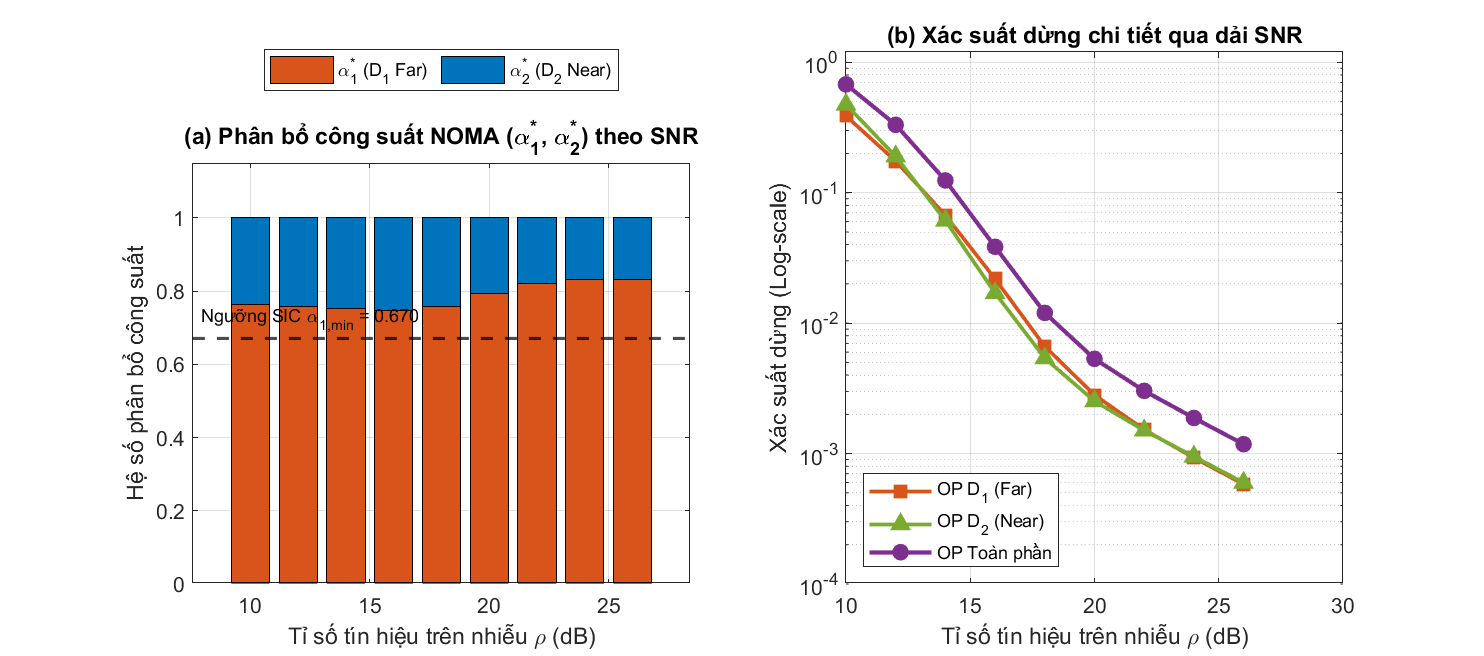
\includegraphics[width=0.86\textwidth]{figures/ao_static_fig4_power_outage.png}
    \caption{Phân bổ hệ số công suất NOMA ($\alpha_1^*, \alpha_2^*$) và xác suất dừng chi tiết từng người dùng qua dải SNR trong mô hình AO Tĩnh: (a) Phân bổ công suất NOMA với ngưỡng an toàn SIC $\alpha_{1,\min} = 0.670$; (b) Xác suất dừng chi tiết của người dùng xa $D_1$, người dùng gần $D_2$ và toàn phần hệ thống.}
    \label{fig:ao_static_power}
\end{figure}

\begin{figure}[H]
    \centering
    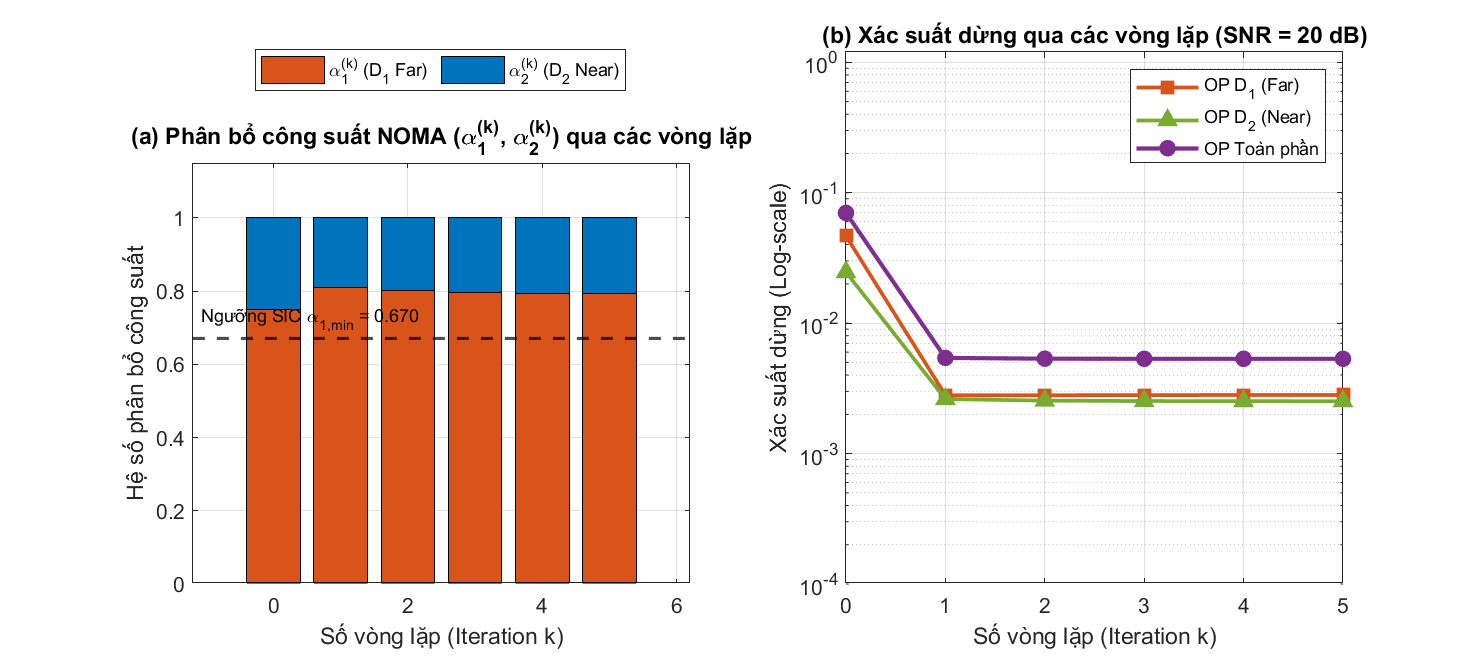
\includegraphics[width=0.86\textwidth]{figures/ao_static_fig5_power_convergence.png}
    \caption{Tiến trình thích ứng hệ số công suất NOMA và suy giảm xác suất dừng qua các vòng lặp hội tụ của thuật toán AO tại $\text{SNR} = 20\text{ dB}$: (a) Sự biến thiên và ổn định của $(\alpha_1^{(k)}, \alpha_2^{(k)})$; (b) Mức suy giảm xác suất dừng thành phần và toàn mạng.}
    \label{fig:ao_static_power_conv}
\end{figure}

\vspace{0.1cm}
\textbf{Phân tích đặc tính phân bổ công suất NOMA trong mô hình AO Tĩnh:}
\begin{itemize}[leftmargin=1.5em]
    \item \textbf{Tuân thủ điều kiện an toàn SIC (Hình \ref{fig:ao_static_power}a):} Trên toàn bộ dải SNR từ $10\text{ dB}$ đến $26\text{ dB}$, hệ số phân bổ công suất cho người dùng xa $D_1$ luôn được duy trì ở mức $\alpha_1^* \in [0.746, 0.832]$, vượt trội so với ngưỡng an toàn SIC giải tích $\alpha_{1,\min} = \frac{\gamma_{th1}}{1 + \gamma_{th1}} \approx 0.670$. Điều này bảo đảm người dùng gần $D_2$ luôn giải mã và loại bỏ can nhiễu tín hiệu của $D_1$ thành công trước khi tách tín hiệu của chính mình.
    \item \textbf{Cân bằng độ tin cậy giữa hai người dùng (Hình \ref{fig:ao_static_power}b):} Nhờ phân bổ công suất thích ứng theo mức SNR, xác suất dừng của cả $D_1$ và $D_2$ đều giảm đều theo hàm mũ. Tại dải SNR cao ($\ge 22\text{ dB}$), do người dùng xa $D_1$ chịu suy hao cự ly lớn hơn đáng kể so với $D_2$, thuật toán giữ tỷ trọng $\alpha_1^* \approx 0.83$ để bảo đảm độ tin cậy kết nối cho $D_1$ mà không làm nghẽn kênh của $D_2$.
    \item \textbf{Tốc độ hội tụ công suất nhanh chóng (Hình \ref{fig:ao_static_power_conv}):} Tại mức SNR thiết kế $20\text{ dB}$, cặp hệ số công suất chuyển dịch mượt mà từ giá trị khởi tạo ban đầu ($\alpha_1^{(0)} = 0.75$) đến điểm tối ưu ổn định ($\alpha_1^* = 0.7948, \alpha_2^* = 0.2052$) chỉ trong $5$ vòng lặp, đồng thời xác suất dừng toàn mạng giảm mạnh từ $7.01 \times 10^{-2}$ xuống $5.33 \times 10^{-3}$ (mức giảm đạt $92.4\%$).
\end{itemize}

% -------------------------------------------------------------------------
\subsection*{2. Kết quả Mô phỏng Tối ưu hóa Luân phiên Động}
Mô hình AO Động học mở rộng bài toán tối ưu trên toàn bộ hành trình gồm $N = 10$ khe thời gian rời rạc, thiết lập nghiệm tham chiếu đối chuẩn (Numerical Benchmark) cho toàn bộ hệ thống SAGIN-NOMA:

\begin{figure}[H]
    \centering
    \begin{subfigure}[b]{0.49\textwidth}
        \centering
        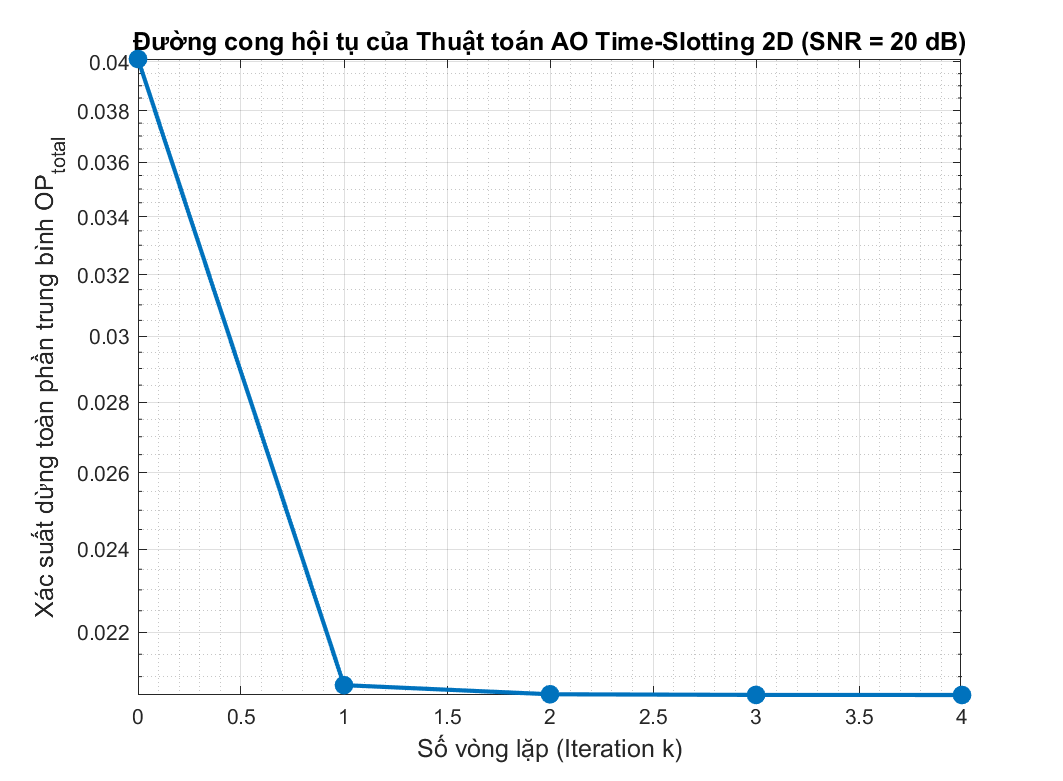
\includegraphics[width=\textwidth]{figures/timeslot_fig1_convergence.png}
        \caption{Đặc tính hội tụ của thuật toán AO Time-Slotting ($\text{SNR} = 20\text{ dB}$)}
        \label{fig:timeslot_conv}
    \end{subfigure}
    \hfill
    \begin{subfigure}[b]{0.49\textwidth}
        \centering
        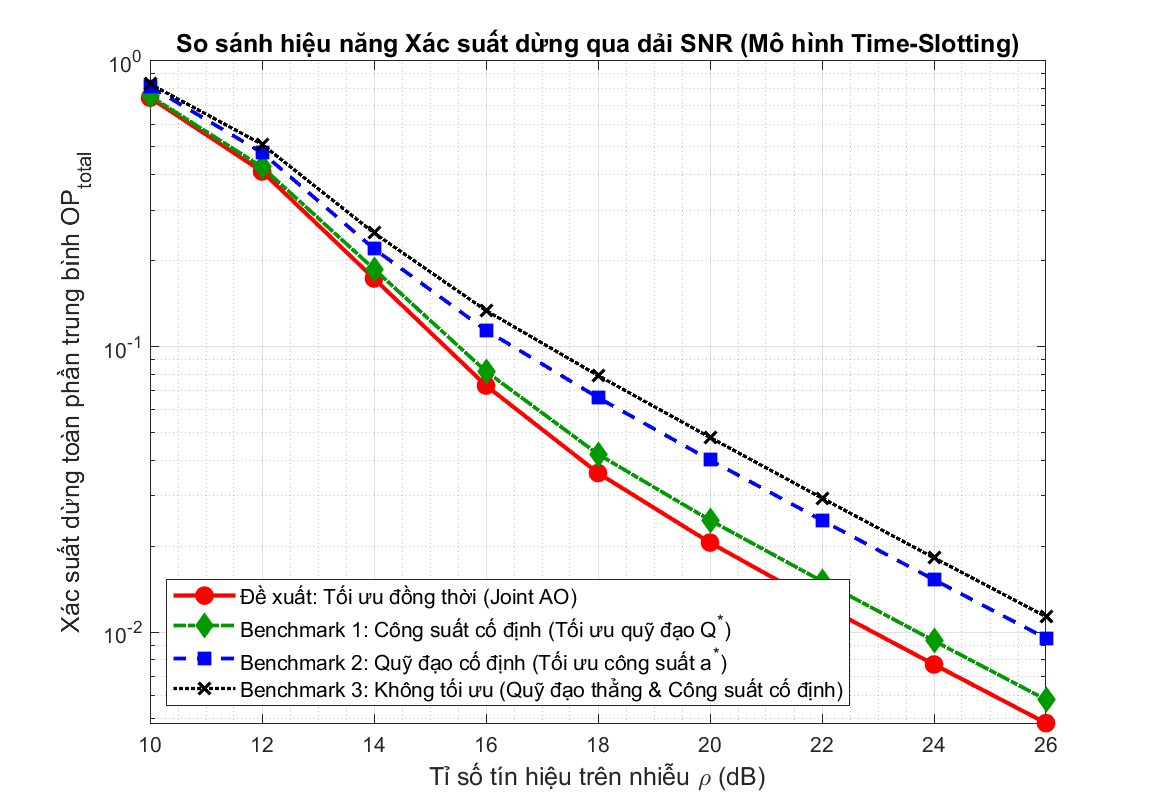
\includegraphics[width=\textwidth]{figures/timeslot_fig2_snr.png}
        \caption{Đối chuẩn xác suất dừng trung bình qua dải SNR giữa Đề xuất và các Benchmark}
        \label{fig:timeslot_snr}
    \end{subfigure}
    \caption{Đặc tính hội tụ nhanh chóng và hiệu năng của thuật toán AO Động Time-Slotting.}
    \label{fig:timeslot_group1}
\end{figure}

\begin{figure}[H]
    \centering
    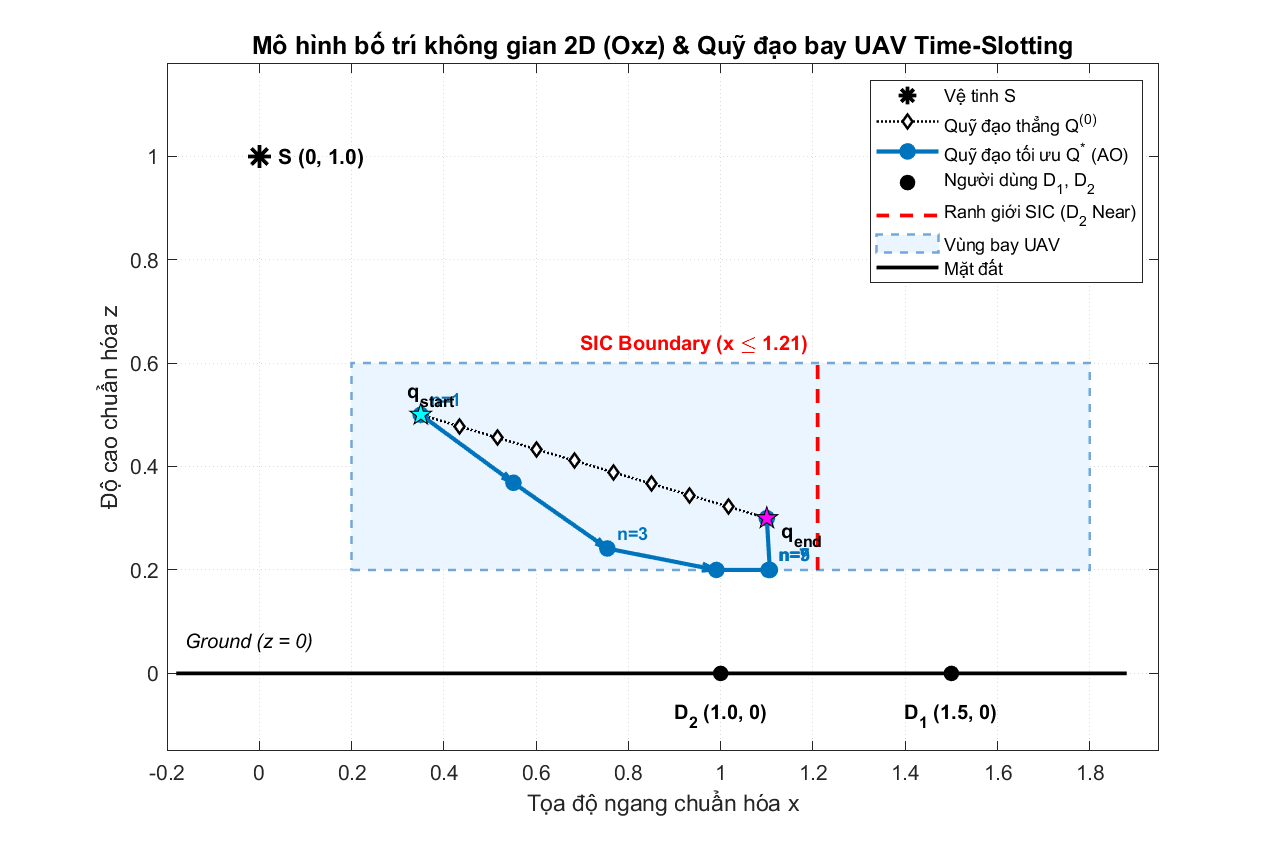
\includegraphics[width=0.86\textwidth]{figures/timeslot_fig3_trajectory.png}
    \caption{Mô hình bố trí không gian 2D $(Oxz)$ và quỹ đạo bay tối ưu của UAV qua $N=10$ khe thời gian tuân thủ nghiêm ngặt ranh giới an toàn SIC $x \le 1.21$.}
    \label{fig:timeslot_traj}
\end{figure}

\begin{figure}[H]
    \centering
    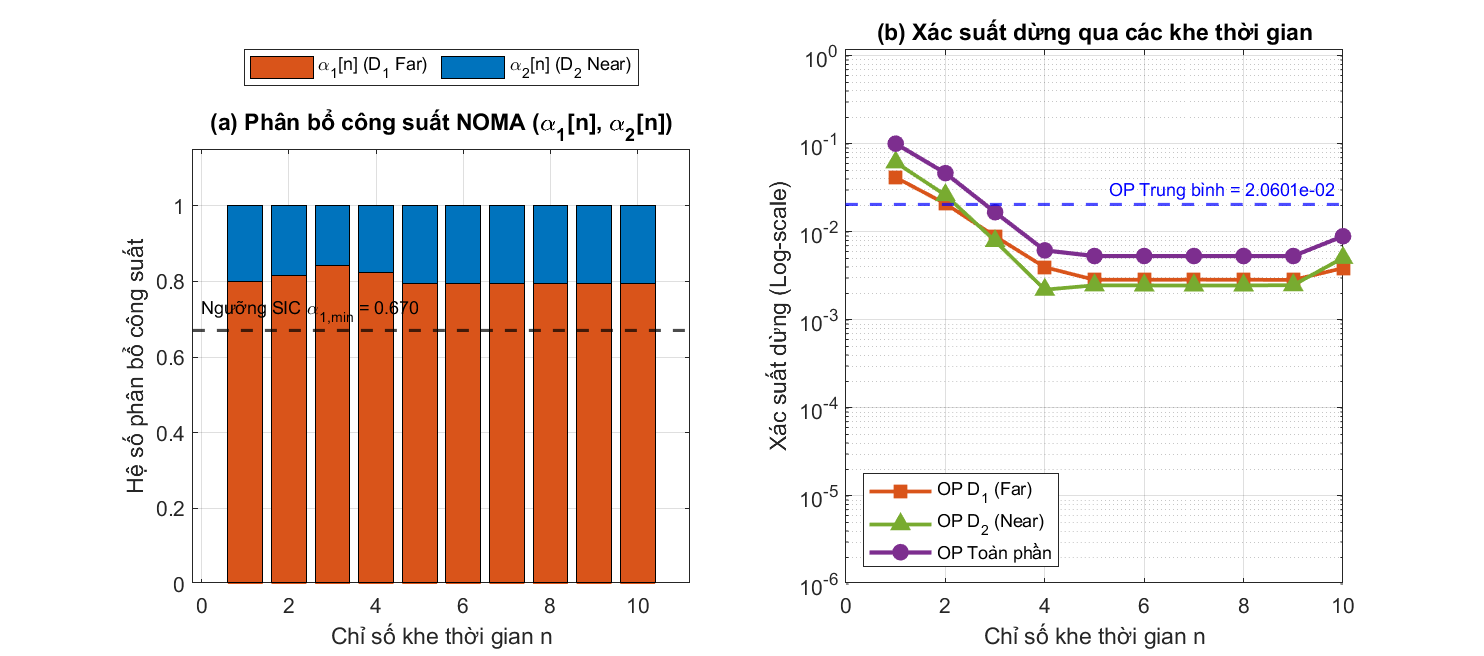
\includegraphics[width=0.86\textwidth]{figures/timeslot_fig4_power_outage.png}
    \caption{Chi tiết phân bổ hệ số công suất NOMA và xác suất dừng qua từng khe thời gian: (a) Phân bổ công suất $(\alpha_1[n], \alpha_2[n])$ thỏa mãn ngưỡng $\alpha_{1,\min} = 0.670$; (b) Xác suất dừng của $D_1$, $D_2$ và toàn phần hệ thống qua từng khe.}
    \label{fig:timeslot_power_outage}
\end{figure}

\vspace{0.1cm}
\textbf{Phân tích đặc tính tối ưu hóa động học không - thời gian:}
\begin{itemize}[leftmargin=1.5em]
    \item \textbf{Đặc tính hội tụ của giải thuật liên hợp (Hình \ref{fig:timeslot_conv}):} Thuật toán AO động học tối ưu luân phiên giữa chuỗi tọa độ quỹ đạo bay $\mathbf{Q}^* \in \mathbb{R}^{10 \times 2}$ và chuỗi hệ số công suất $\boldsymbol{\alpha}_1^* \in \mathbb{R}^{10}$. Hàm mục tiêu xác suất dừng toàn phần trung bình giảm ngặt từ giá trị ban đầu $4.01 \times 10^{-2}$ xuống đáy tối ưu $2.06 \times 10^{-2}$ chỉ sau $4$ vòng lặp SQP kết hợp Penalty.
    \item \textbf{Hiệu năng đối chuẩn toàn diện theo SNR (Hình \ref{fig:timeslot_snr}):} Giải pháp tối ưu đồng thời Joint AO Time-Slotting (đường đỏ) luôn đạt xác suất dừng thấp nhất trên toàn bộ dải SNR từ $10\text{ dB}$ đến $26\text{ dB}$, vượt trội so với kịch bản chỉ tối ưu quỹ đạo (Benchmark 1, xanh lá), chỉ tối ưu công suất (Benchmark 2, xanh dương) và kịch bản không tối ưu (Benchmark 3, đen nét chấm).
    \item \textbf{Quỹ đạo bay thích ứng tuân thủ ranh giới an toàn SIC (Hình \ref{fig:timeslot_traj}):} Xuất phát từ $\mathbf{q}_{\text{start}}(0.35, 0.50)$, UAV bay hạ thấp độ cao và lượn gần về phía người dùng gần $D_2(1.0, 0)$ nhưng luôn giữ khoảng cách an toàn trước ranh giới hình học SIC $x \le 1.21$ để bảo đảm thứ tự giải mã can nhiễu không bị đảo lộn, sau đó cơ động chuẩn xác về đích $\mathbf{q}_{\text{end}}(1.10, 0.30)$ ở khe cuối cùng $n = 10$.
    \item \textbf{Chiến lược phân bổ công suất động theo từng vị trí bay (Hình \ref{fig:timeslot_power_outage}):} Tại khe đầu $n=1$, do UAV nằm cố định tại điểm xuất phát $q_{\text{start}}$, xác suất dừng đạt mức cao nhất ($OP[1] \approx 0.1008$). Tại các khe giữa ($n = 4 \to 8$), khi UAV tiếp cận gần $D_2$, kênh truyền chặng 2 được cải thiện đáng kể, xác suất dừng toàn phần tại các khe này giảm sâu xuống mức xấp xỉ $5.3 \times 10^{-3}$ (trong đó xác suất dừng của riêng người dùng gần $D_2$ chạm mức $2.1 \times 10^{-3}$).
\end{itemize}

% -------------------------------------------------------------------------
\subsection*{3. Kết quả Mô phỏng Học tăng cường sâu Thời gian thực (Real-Time DRL Agent)}
Tác tử DRL sử dụng thuật toán Deep Deterministic Policy Gradient (DDPG) Actor-Critic tự chủ ra quyết định điều khiển quỹ đạo và phân bổ công suất theo thời gian thực ở cấp độ mili-giây, giải quyết điểm nghẽn độ trễ tính toán của phương pháp AO:

\begin{figure}[H]
    \centering
    \begin{subfigure}[b]{0.49\textwidth}
        \centering
        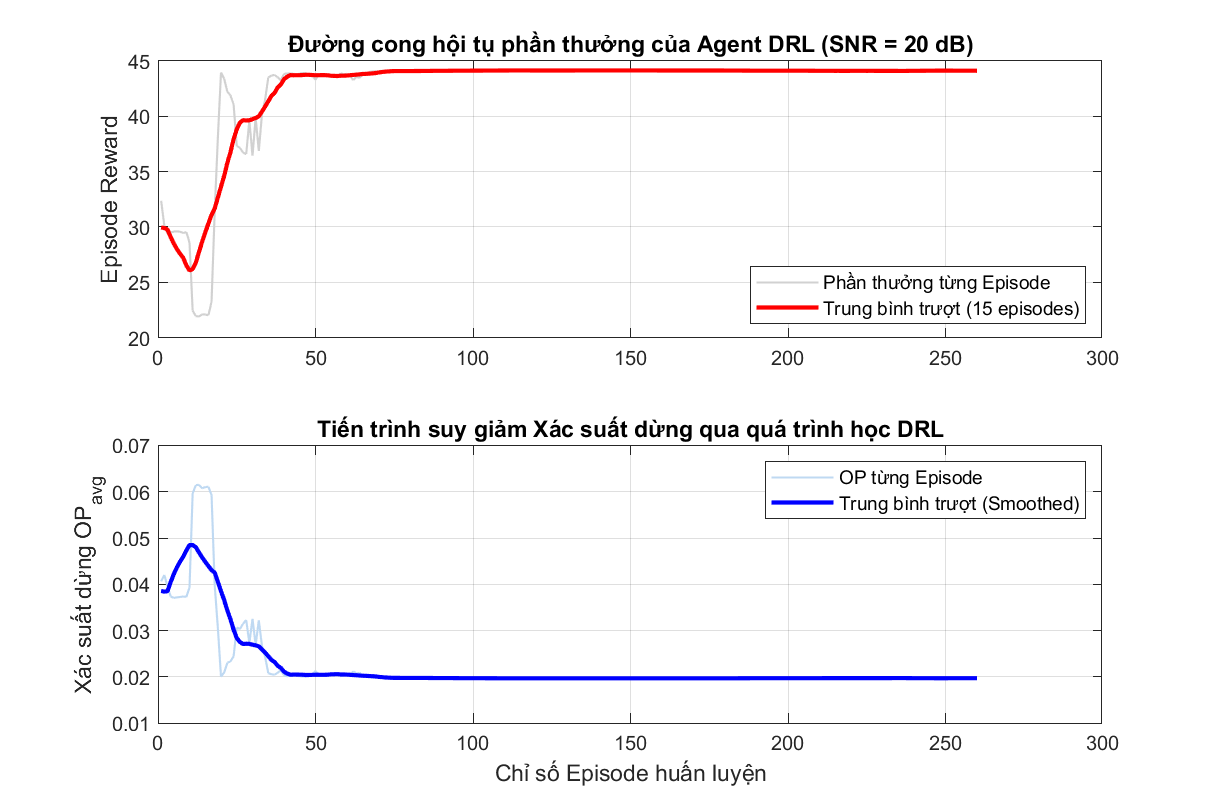
\includegraphics[width=\textwidth]{figures/drl_fig1_convergence.png}
        \caption{Đặc tính hội tụ phần thưởng và suy giảm OP qua các Episode huấn luyện DRL}
        \label{fig:drl_conv}
    \end{subfigure}
    \hfill
    \begin{subfigure}[b]{0.49\textwidth}
        \centering
        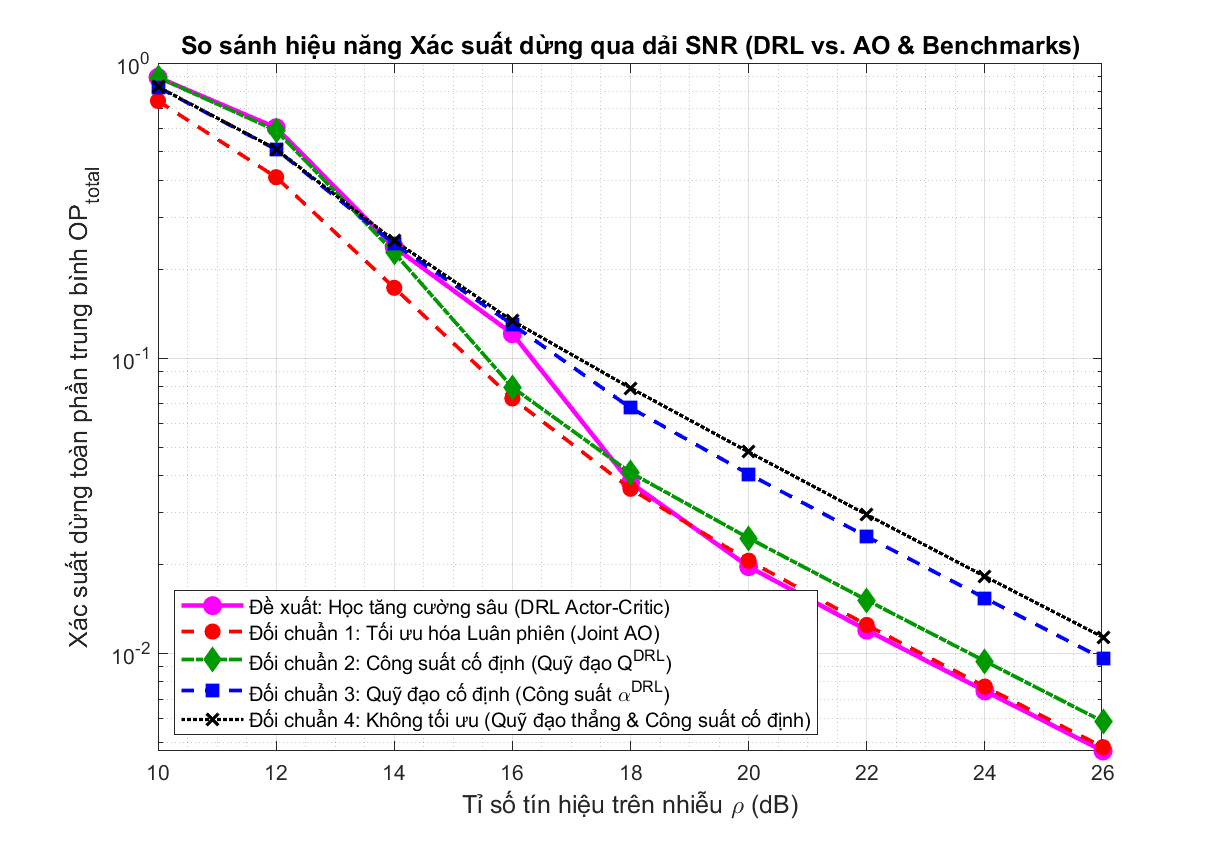
\includegraphics[width=\textwidth]{figures/drl_fig2_snr.png}
        \caption{Đối chuẩn xác suất dừng qua dải SNR giữa DRL, Joint AO và các Benchmark}
        \label{fig:drl_snr}
    \end{subfigure}
    \caption{Đặc tính huấn luyện ổn định và hiệu năng tiệm cận mốc tham chiếu chuẩn của tác tử DRL Actor-Critic.}
    \label{fig:drl_group1}
\end{figure}

\begin{figure}[H]
    \centering
    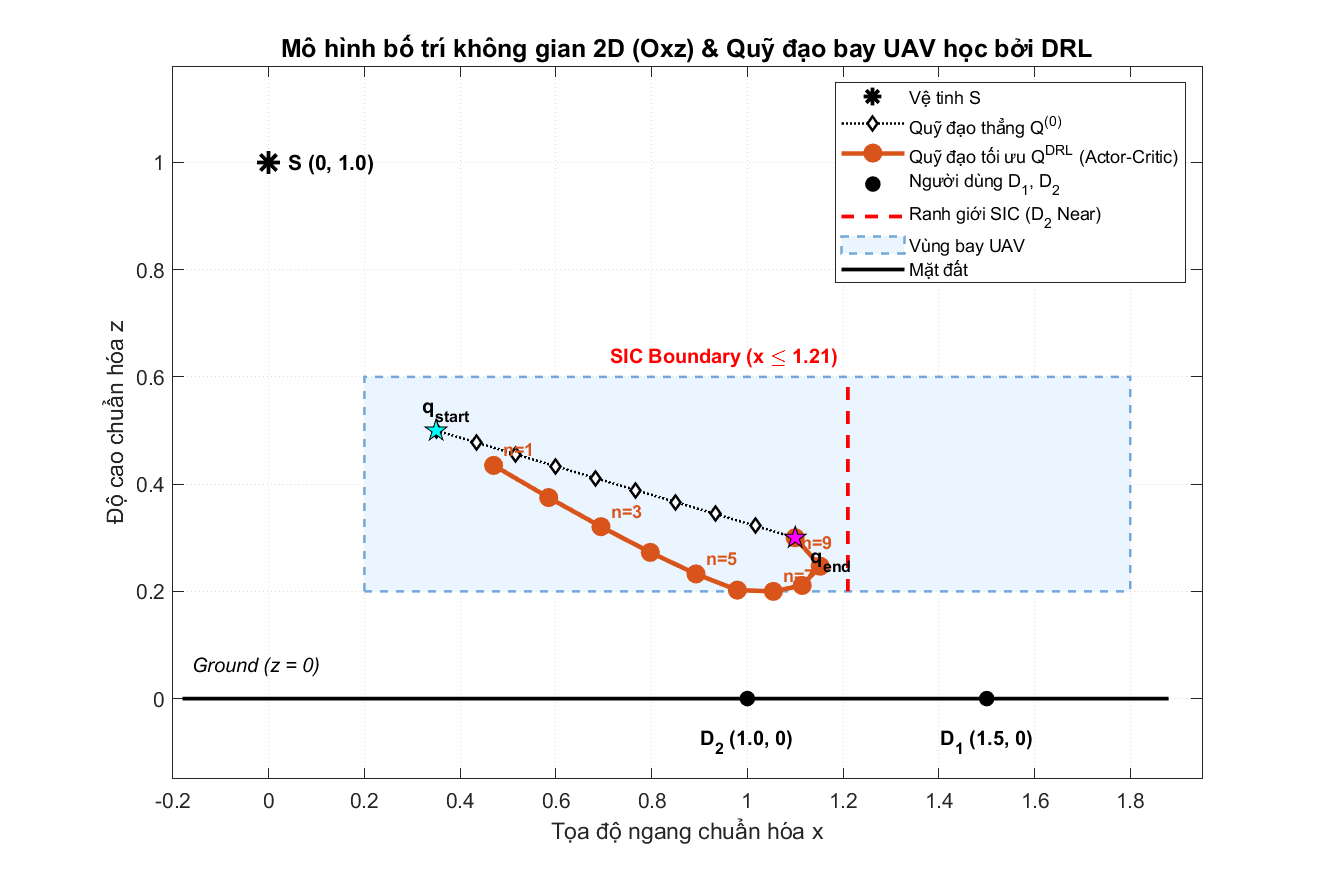
\includegraphics[width=0.86\textwidth]{figures/drl_fig3_trajectory.png}
    \caption{Mô hình bố trí không gian 2D $(Oxz)$ và quỹ đạo bay UAV do mạng DRL tự chủ điều hướng qua $N=10$ bước bay, duy trì vùng đệm an toàn cách ranh giới SIC $x \le 1.21$ và hạ cánh tại đích $q_{\text{end}}$.}
    \label{fig:drl_traj}
\end{figure}

\begin{figure}[H]
    \centering
    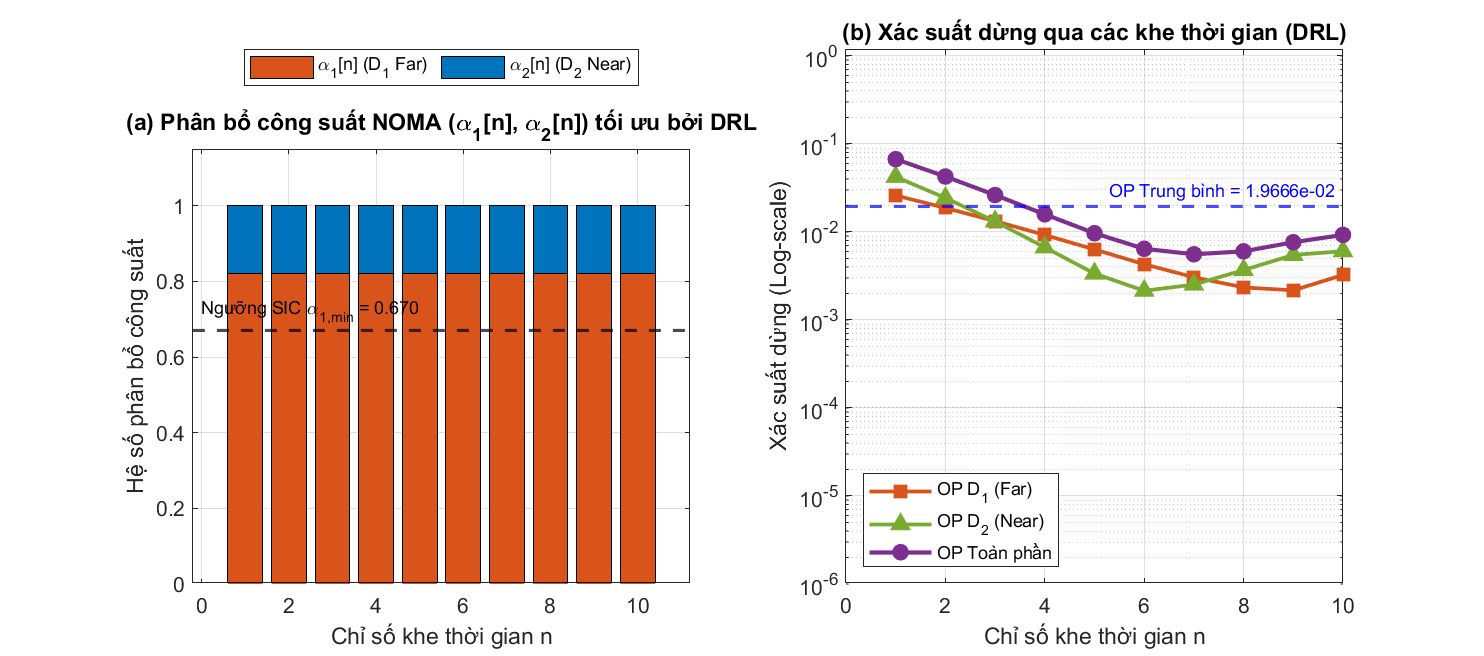
\includegraphics[width=0.86\textwidth]{figures/drl_fig4_power_outage.png}
    \caption{Chi tiết phân bổ hệ số công suất NOMA và xác suất dừng qua các khe thời gian được suy luận bởi tác tử DRL: (a) Phân bổ công suất $(\alpha_1[n], \alpha_2[n])$ thời gian thực; (b) Xác suất dừng chi tiết từng khe.}
    \label{fig:drl_power_outage}
\end{figure}

\vspace{0.1cm}
\textbf{Phân tích đặc tính điều khiển thời gian thực và tự thích ứng của DRL:}
\begin{itemize}[leftmargin=1.5em]
    \item \textbf{Quá trình huấn luyện bền vững (Hình \ref{fig:drl_conv}):} Nhờ cơ chế gieo mẫu kinh nghiệm khởi động ấm (Warm-Start Experience Seeding -- nạp các chuyển tiếp mẫu từ đường bay thẳng ban đầu vào Replay Buffer) và dẫn hướng dịch chuyển (Guided Displacement), phần thưởng tích lũy trung bình mỗi tập (Episode Reward) tăng đều đặn từ khoảng $25$ lên ổn định ở mức $\approx 44$, trong khi xác suất dừng trung bình giảm sâu và ổn định tiệm cận ngưỡng tối ưu chỉ sau $\approx 50$ episodes mà không bị phân kỳ.
    \item \textbf{Hiệu năng đối chuẩn qua dải SNR (Hình \ref{fig:drl_snr}):} Tác tử DRL được huấn luyện tại mức SNR danh định $20\text{ dB}$, sau đó được đánh giá trực tiếp (zero-shot) trên toàn dải SNR từ $10\text{ dB}$ đến $26\text{ dB}$. Tại vùng SNR cao ($\ge 18\text{ dB}$), DRL bám rất sát và đạt hiệu năng tương đương nghiệm số học của AO Động ($0.0197$ so với $0.0206$ tại $20\text{ dB}$). Tại vùng SNR thấp ($10 \to 16\text{ dB}$), đường cong DRL cao hơn nhẹ so với AO do chính sách mạng nơ-ron được tối ưu hóa chuyên biệt tại điều kiện kênh $20\text{ dB}$, thể hiện đặc tính đánh giá ngoài phân bố huấn luyện thông thường.
    \item \textbf{Điều hướng mượt mà và tự bảo vệ an toàn SIC (Hình \ref{fig:drl_traj}):} Mạng Actor học được chính sách điều khiển liên tục, tạo ra quỹ đạo bay mượt mà, chủ động giữ cự ly an toàn đệm khoảng $0.06$ đơn vị cách mép ranh giới SIC ($x \le 1.21$) để tránh vi phạm thứ tự người dùng. Tại bước $n=10$, tác tử hạ cánh chính xác tại tọa độ đích $q_{\text{end}}(1.10, 0.30)$.
    \item \textbf{Phân bổ công suất thích ứng linh hoạt (Hình \ref{fig:drl_power_outage}):} Tác tử DRL liên tục cập nhật hệ số công suất $\alpha_1[n] \in [0.78, 0.83]$ (trung bình $0.820$) tương ứng với từng tọa độ bay thực tế, giúp xác suất dừng toàn mạng tại các khe giữa $n = 5 \to 8$ giảm xuống mức $\approx 5.6 \times 10^{-3} - 9.7 \times 10^{-3}$, hoàn toàn phù hợp với mức trung bình $0.0197$ trên toàn hành trình.
    \item \textbf{Ưu thế thời gian suy luận trực tuyến (1.5 ms):} Ưu thế thực tiễn nổi bật của DRL là thời gian ra quyết định tức thời chỉ $\mathbf{1.5}$ mili-giây cho mỗi bước bay (tổng $15$ ms cho toàn hành trình), nhanh hơn $\mathbf{120}$ lần so với tổng thời gian giải lặp của AO Động ($1850$ ms). Khả năng tính toán siêu nhanh này là nền tảng cốt lõi cho phép điều khiển bay trực tuyến trên các thiết bị nhúng hạn chế năng lượng của UAV.
\end{itemize}
